\documentclass[aspectratio=169,11pt]{beamer}
\usepackage[T1]{fontenc}
\usepackage{lmodern,amsmath,amssymb,mathtools,bm,booktabs,array,graphicx,tikz}
\usetikzlibrary{arrows.meta,positioning,calc,decorations.pathreplacing,patterns}
\definecolor{ink}{HTML}{17344D}\definecolor{accent}{HTML}{087E8B}\definecolor{pale}{HTML}{EDF5F5}\definecolor{gold}{HTML}{AD6B19}
\providecommand{\dd}{\,\mathrm{d}}\providecommand{\R}{\mathbb{R}}
\providecommand{\E}{\mathbb{E}}\providecommand{\Var}{\operatorname{Var}}
\providecommand{\Cov}{\operatorname{Cov}}\providecommand{\diag}{\operatorname{diag}}
\providecommand{\norm}[1]{\left\lVert#1\right\rVert}
\providecommand{\abs}[1]{\left|#1\right|}
\usefonttheme{professionalfonts}
\setbeamercolor{normal text}{fg=black,bg=white}
\setbeamercolor{frametitle}{fg=ink,bg=white}
\setbeamercolor{title}{fg=ink}\setbeamercolor{structure}{fg=accent}
\setbeamercolor{block title}{fg=ink,bg=pale}\setbeamercolor{block body}{fg=black,bg=pale!40}
\setbeamercolor{alerted text}{fg=accent}
\setbeamerfont{frametitle}{size=\Large,series=\bfseries}
\setbeamerfont{title}{size=\LARGE,series=\bfseries}
\setbeamertemplate{navigation symbols}{}
\setbeamersize{text margin left=.7cm,text margin right=.7cm}
\setbeamertemplate{frametitle}{\vspace{.18cm}\insertframetitle\par\vspace{.1cm}{\color{accent}\hrule height .6pt}\vspace{.12cm}}
\newcommand{\notestarget}{notes.pdf}\newcommand{\noteslabel}{Notes}
\setbeamertemplate{footline}{\hspace{.7cm}\color{ink}\scriptsize Computational Cardiology\quad\href{\notestarget}{\noteslabel}\hfill\insertframenumber\,/\,\inserttotalframenumber\hspace{.7cm}\vspace{.18cm}}
\setbeamercovered{invisible}
\hypersetup{pdfauthor={Zan Ahmad},pdftitle={Field errors, conserved moments and correlation invariance},pdfpagemode=UseNone}
\begin{document}
\begin{frame}[plain]\vfill
{\small\color{accent} Computational Cardiology \quad Lecture 20}\par\medskip
{\raggedright\hyphenpenalty=10000\exhyphenpenalty=10000\LARGE\bfseries\color{ink} Field errors, conserved moments and correlation invariance}\par\bigskip
Zan Ahmad\par\smallskip
{\small Fall 2024}\par\vfill\end{frame}
\renewcommand{\notestarget}{notes.pdf\#note-equations-and-observables-in-a-scientific-argument}
\begin{frame}[t,fragile,label=slide-an-observable-selects-part-of-a-solution]{An observable selects part of a solution}
Mean flow, total volume, arrival time and correlation summarize different features.\pause{} Agreement in one does not determine the complete state or field.
\end{frame}
\renewcommand{\notestarget}{notes.pdf\#note-field-error-and-aggregate-summaries}
\begin{frame}[label=slide-two-explicit-candidate-fields-panel-1]{A field metric sees both failures}
\centering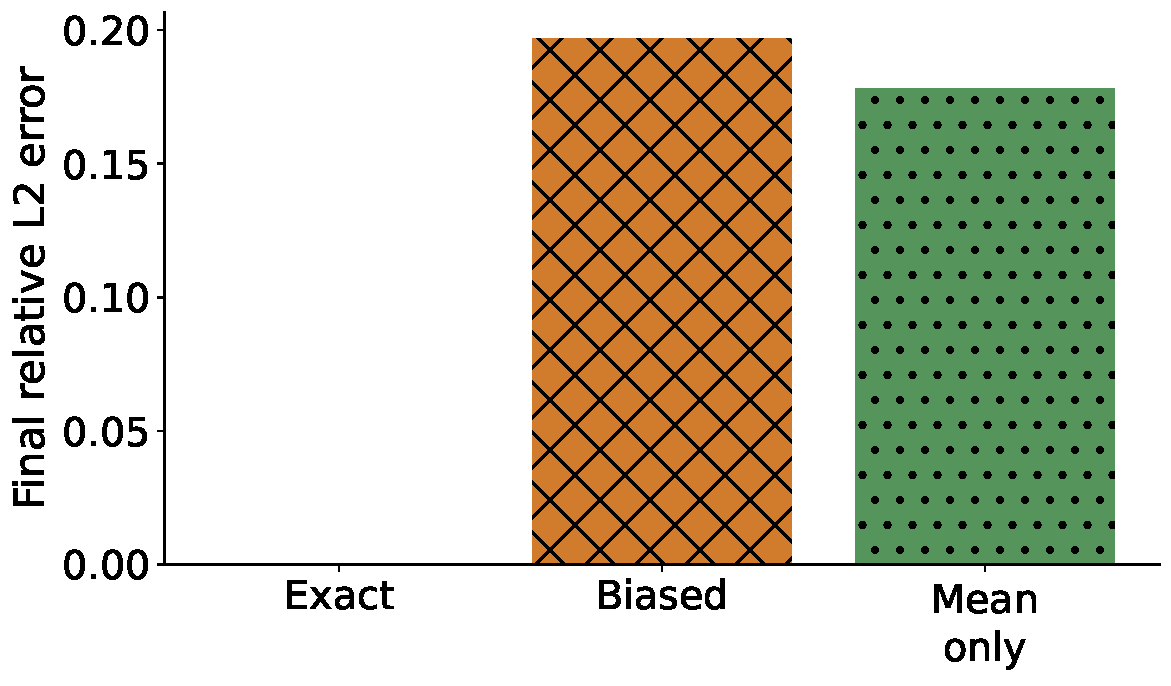
\includegraphics[width=.98\linewidth,height=.69\textheight,keepaspectratio]{presentation-figures/evidence-audit-panel-1.pdf}\end{frame}
\renewcommand{\notestarget}{notes.pdf\#note-field-error-and-aggregate-summaries}
\begin{frame}[label=slide-two-explicit-candidate-fields-panel-2]{Correlation can miss a bias}
\centering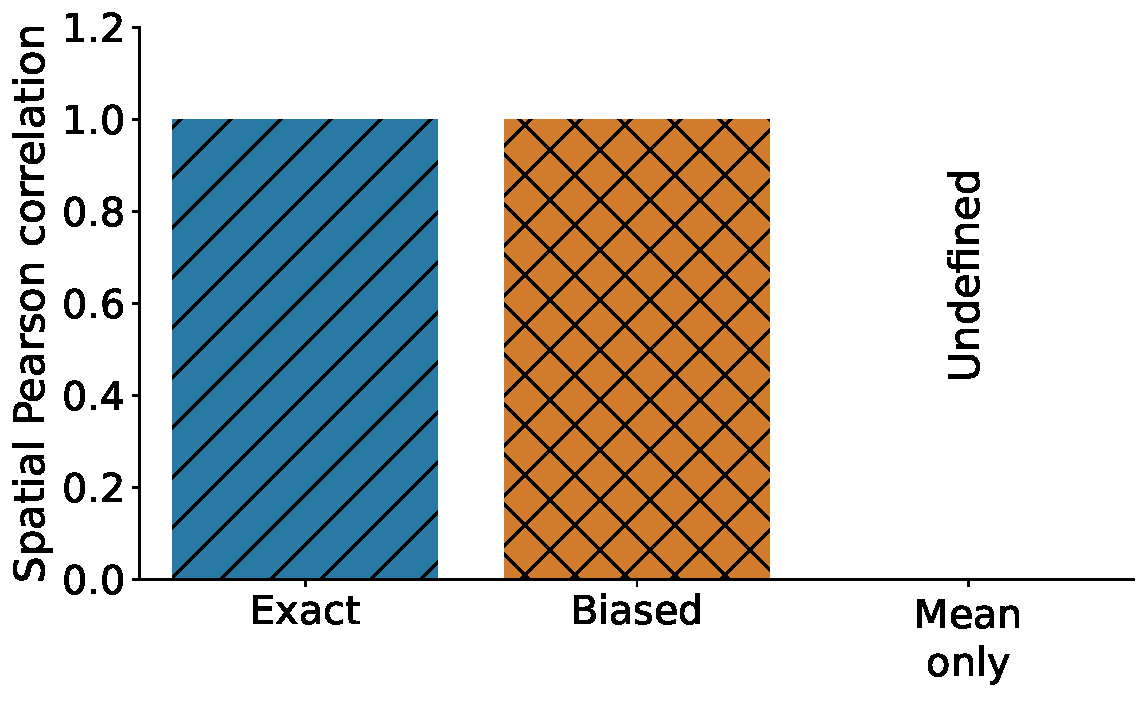
\includegraphics[width=.98\linewidth,height=.69\textheight,keepaspectratio]{presentation-figures/evidence-audit-panel-2.pdf}\end{frame}
\renewcommand{\notestarget}{notes.pdf\#note-field-error-and-aggregate-summaries}
\begin{frame}[t,fragile,label=slide-two-explicit-candidate-fields]{Two explicit candidate fields}
\[p_{bias}(x,t)=u(x,t)+.2,\qquad p_{mean}(x,t)=\overline u(t).\]\pause{} The exact sealed heat trajectory supplies a common reference.
\end{frame}
\renewcommand{\notestarget}{notes.pdf\#note-field-error-and-aggregate-summaries}
\begin{frame}[t,fragile,label=slide-absolute-rms-error]{Absolute RMS error}
\[E_{RMS}=\left(\frac1N\sum_i(p_i-y_i)^2\right)^{1/2}.\]\pause{} A constant offset $b$ gives $E_{RMS}=|b|$.
\end{frame}
\renewcommand{\notestarget}{notes.pdf\#note-field-error-and-aggregate-summaries}
\begin{frame}[t,fragile,label=slide-relative-error-needs-a-nonzero-reference-norm]{Relative error needs a nonzero reference norm}
\[E_{rel}=\frac{\|p-y\|}{\|y\|}.\]\pause{} If $\|y\|=0$, this quotient is undefined without a separate convention.
\end{frame}
\renewcommand{\notestarget}{notes.pdf\#note-affine-invariance-of-pearson-correlation}
\begin{frame}[t,fragile,label=slide-pearson-correlation]{Pearson correlation}
\[\rho(p,y)=\frac{(p-\bar p\boldsymbol1)^{\mathsf T}(y-\bar y\boldsymbol1)}{\|p-\bar p\boldsymbol1\|\,\|y-\bar y\boldsymbol1\|}.\]\pause{} Both centered norms must be nonzero.
\end{frame}
\renewcommand{\notestarget}{notes.pdf\#note-affine-invariance-of-pearson-correlation}
\begin{frame}[t,fragile,label=slide-center-an-affine-prediction]{Center an affine prediction}
\[p=ay+b\boldsymbol1\quad\Longrightarrow\quad p-\bar p\boldsymbol1=a(y-\bar y\boldsymbol1).\]\pause{} The offset disappears.
\end{frame}
\renewcommand{\notestarget}{notes.pdf\#note-affine-invariance-of-pearson-correlation}
\begin{frame}[t,fragile,label=slide-correlation-ignores-positive-rescaling]{Correlation ignores positive rescaling}
\[\rho(ay+b\boldsymbol1,y)=\operatorname{sign}(a),\qquad a\ne0.\]\pause{} Positive amplitude errors and arbitrary offsets can coexist with correlation one.
\end{frame}
\renewcommand{\notestarget}{notes.pdf\#note-affine-invariance-of-pearson-correlation}
\begin{frame}[t,fragile,label=slide-a-hand-calculation]{A hand calculation}
\[y=(1,3,5),\qquad p=(3,5,7).\]\pause{} Both centered vectors are $(-2,0,2)$, while the error is $(2,2,2)$.
\end{frame}
\renewcommand{\notestarget}{notes.pdf\#note-affine-invariance-of-pearson-correlation}
\begin{frame}[t,fragile,label=slide-compatible-but-different-conclusions]{Compatible but different conclusions}
\[\rho=1,\qquad E_{RMS}=2,\qquad\bar p-\bar y=2.\]\pause{} These numbers answer different questions.
\end{frame}
\renewcommand{\notestarget}{notes.pdf\#note-affine-invariance-of-pearson-correlation}
\begin{frame}[t,fragile,label=slide-a-constant-prediction]{A constant prediction}
If $p_i=\bar y$ for every $i$, its mean is correct but its centered norm is zero.\pause{} Correlation is undefined and nonconstant reference structure is lost.
\end{frame}
\renewcommand{\notestarget}{notes.pdf\#note-conservation-and-prescribed-initial-data}
\begin{frame}[label=slide-conservation-relative-to-the-initial-prediction-panel-1]{Three different field claims}
\centering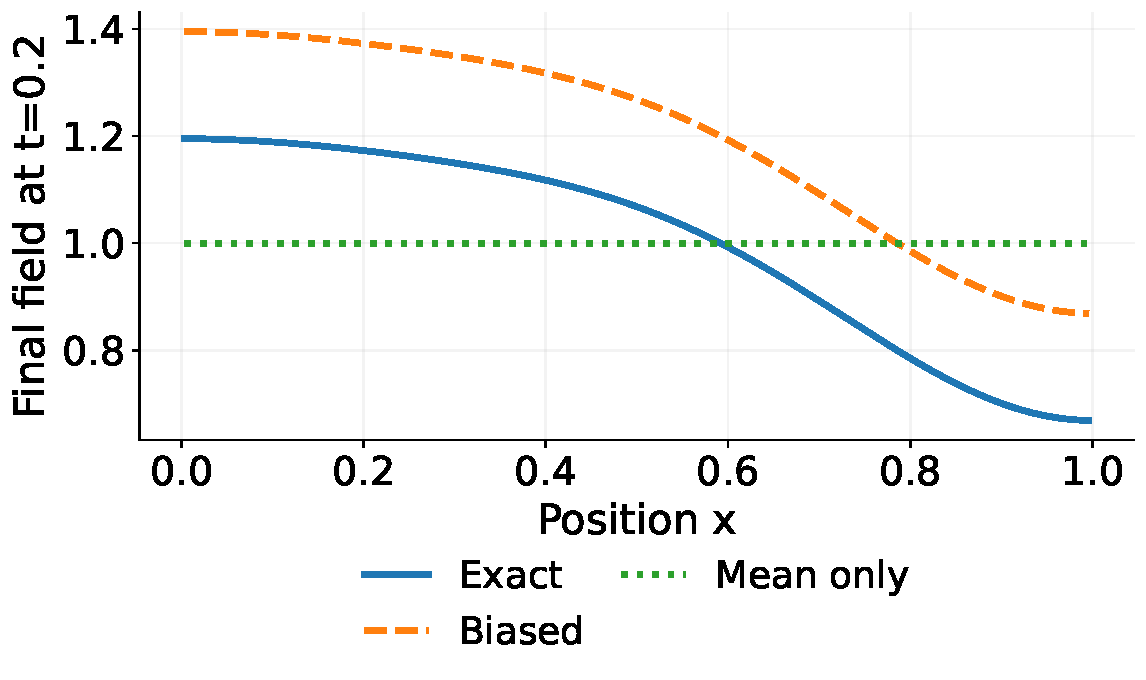
\includegraphics[width=.98\linewidth,height=.69\textheight,keepaspectratio]{presentation-figures/field-and-moment-panel-1.pdf}\end{frame}
\renewcommand{\notestarget}{notes.pdf\#note-conservation-and-prescribed-initial-data}
\begin{frame}[label=slide-conservation-relative-to-the-initial-prediction-panel-2]{Conserved does not mean correct}
\centering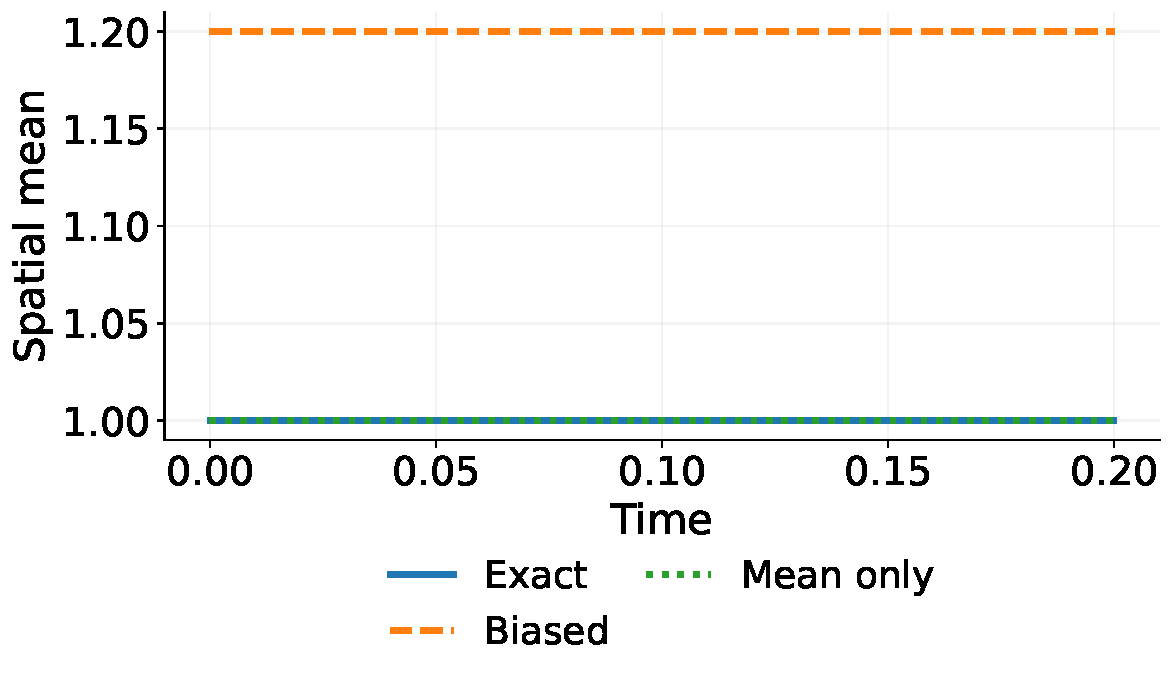
\includegraphics[width=.98\linewidth,height=.69\textheight,keepaspectratio]{presentation-figures/field-and-moment-panel-2.pdf}\end{frame}
\renewcommand{\notestarget}{notes.pdf\#note-conservation-and-prescribed-initial-data}
\begin{frame}[t,fragile,label=slide-conservation-relative-to-the-initial-prediction]{Conservation relative to the initial prediction}
\[r_{drift}(t)=\overline p(t)-\overline p(0).\]\pause{} An offset candidate can have zero drift throughout the trajectory.
\end{frame}
\renewcommand{\notestarget}{notes.pdf\#note-conservation-and-prescribed-initial-data}
\begin{frame}[t,fragile,label=slide-conservation-for-the-prescribed-problem]{Conservation for the prescribed problem}
\[r_{prescribed}(t)=\overline p(t)-\overline y(0).\]\pause{} For $p=y+b$, this residual equals $b$, exposing the incorrect initial mean.
\end{frame}
\renewcommand{\notestarget}{notes.pdf\#note-orthogonal-error-components}
\begin{frame}[t,fragile,label=slide-orthogonal-decomposition-of-field-error]{Orthogonal decomposition of field error}
\[e=\bar e\boldsymbol1+e_c,\qquad\boldsymbol1^{\mathsf T}e_c=0.\]\pause{}\[\frac1N\|e\|^2=\bar e^2+\frac1N\|e_c\|^2.\]
\end{frame}
\renewcommand{\notestarget}{notes.pdf\#note-orthogonal-error-components}
\begin{frame}[t,fragile,label=slide-what-the-mean-cannot-determine]{What the mean cannot determine}
A mean constraint controls one component of the field error.\pause{} Every nonconstant mode can still be wrong, even when the mean history is exact.
\end{frame}
\renewcommand{\notestarget}{notes.pdf\#note-synthesis-across-models-and-representations}
\begin{frame}[t,fragile,label=slide-a-precise-synthesis]{A precise synthesis}
Conservation constrains balances; alignment constrains allowed pose; arrival times constrain events; field norms constrain amplitudes.\pause{} The mathematical claim should match the observable actually established.
\end{frame}
\end{document}
